\documentstyle[info-utf8,graphicx]{jarticle}
%
% 著者の所属が1つの研究機関の場合の様式
%
%\author{情報太郎\Email{hokkaido@ipsj.or.jp}
%\hspace{5mm}情報次郎
%\hspace{5mm}情報三郎 \\
%(北大情報科学)\contactto{札幌市北区北14条西9丁目北海道大学大学院情報科学研究科}}
%
% 著者が複数の研究機関に所属する場合の様式
%
\author{%
\begin{tabular}{ccc}
武信雄平\Email{b1016127@fun.ac.jp} &
奥野拓 \\
\multicolumn{2}{c}{%
(公立はこだて未来大学)\contactto{北海道函館市亀田中野町116番地2公立はこだて未来大学システム情報科学部}}
\end{tabular}}

\title{観光スポットと移動経路に対する嗜好を考慮した \\
観光ルート推薦システムの構築}

\begin{document}
\maketitle

\section{はじめに}\label{sec:はじめに}
土地勘のない観光客にとって,観光を快適に楽しむためには,事前に観光プランを作成することが重要である.
そのため,WebサイトやSNSなどを利用し,観光に必要な情報の収集や移動手段などを考慮したスケジュールの作成が必要となる.
しかし,WebサイトやSNSなどから観光に必要な情報を見つけることや,移動手段などを考慮してスケジュールを作成することは,観光客にとって負担が大きい.
そのため,観光客の負担が少ない観光プラン作成支援システムが必要である.
観光客に適した観光プランを作成するためには,観光スポットや移動経路に対する嗜好を考慮した観光ルートを作成する必要がある.


本研究では,観光客の観光スポットと移動経路に対する嗜好を考慮した観光プランの作成を支援する.
そのために,満足度が高く,負担の少ない観光ルートを生成することを目指す.

\section{観光ルートの自動生成に関する研究}\label{sec:観光ルートの自動生成に関する研究}
観光客の満足度向上を目的とした先行研究がある\cite{倉田}.
この研究では,ユーザの観光スポットに対する嗜好をもとにした観光ルートの自動生成と,対話的なルート変更が可能なシステムを構築している.
このシステムでは,ユーザがレーダーチャートを操作することにより,自らの嗜好を直接入力する.
さらに,観光したい,もしくはしたくない場所をユーザが設定できる.
しかし,移動経路に対する嗜好は考慮されていない.
移動経路に対する嗜好とは,観光や移動にかける時間,費用などをどの程度重視するかのことである.


他に,ユーザの要求に合った観光ルートを選択するための意思決定を支援することを目的とした先行研究がある\cite{平野}.
この研究では,ユーザの嗜好と消費するリソースを考慮した複数の観光ルート提示手法を提案している.
この研究の提案手法では,観光の満足度とユーザが移動や観光地で消費するリソースを考慮し,パレート最適解となる観光ルートを生成する.
ここで挙げている消費リソースは,金銭,時間,体力の3項目である.
その後,生成した観光ルートを複数提示し,ユーザがその中からルートを選択する.
しかし,各項目に対して重みづけがされていないため,観光スポットと移動経路に対するユーザの嗜好の一部を強く優先したルートを生成できない.

\section{観光ルート自動生成システム}\label{sec:観光ルート自動生成システム}
本研究では,観光スポットと移動経路に対するユーザの嗜好の一部を強く優先したルートを自動生成するためのシステムを構築する.
システムのイメージをFig.\ref{fig:観光ルート表示画面}に示す.
構築するシステムでは,初めにユーザに出発地点,到着地点を入力してもらう.
入力方法は2つある.
一つは各地点名をテキストでの入力する方法,もう一つは地図上から任意の位置を選択する方法である.
その他に,出発時刻,到着時刻も入力してもらう.
それらの入力後,どのような観光スポットや移動経路,方法が好みであるかを入力してもらう.
その際,入力には各特徴のスライダーを操作してもらい,直感的に入力してもらう.
ここでいう特徴とは,観光スポットや移動経路,方法のことである.
その後,ユーザの入力内容を基に,ルートを自動で生成する.
ルートの生成方法については,\ref{sec:観光ルート自動生成アルゴリズム}章にて記述する.
その後,生成されたルートからいくつかの特徴が異なるルートを表示する.
その中から1つを選択すると,そのコースの特徴と,どのようなスケジュールで観光スポットを回るかを表示する.
その際地図上では,移動経路と観光スポットの位置を表示する.
また,表示されている観光スポット名を選択すると,地図部分の代わりに選択された観光スポットの情報を表示する.
表示されたルートのいずれかをユーザが気に入った場合は,そのルートのスケジュール下部にある”このルートにする”を選択してもらう.
表示されたルートとは異なる特徴を持つルートを知りたい場合は,”別のルートを表示する”を選択してもらう.
表示されているルートを改善したルートを知りたい場合,改善したいルートのスケジュール下部にある”このルートの一部を改善したルートを新たに作成する”ボタンを選択してもらう.
その後,改善したい部分をチェックボックスを用いて選択してもらい,それに合わせたルートの生成を再度行う.
生成されたルートは再度Fig.\ref{fig:観光ルート表示画面}のように表示する.
これらをユーザが気に入ったコースが表示されるまで繰り返す.
\begin{figure}[h]
  \begin{center}
  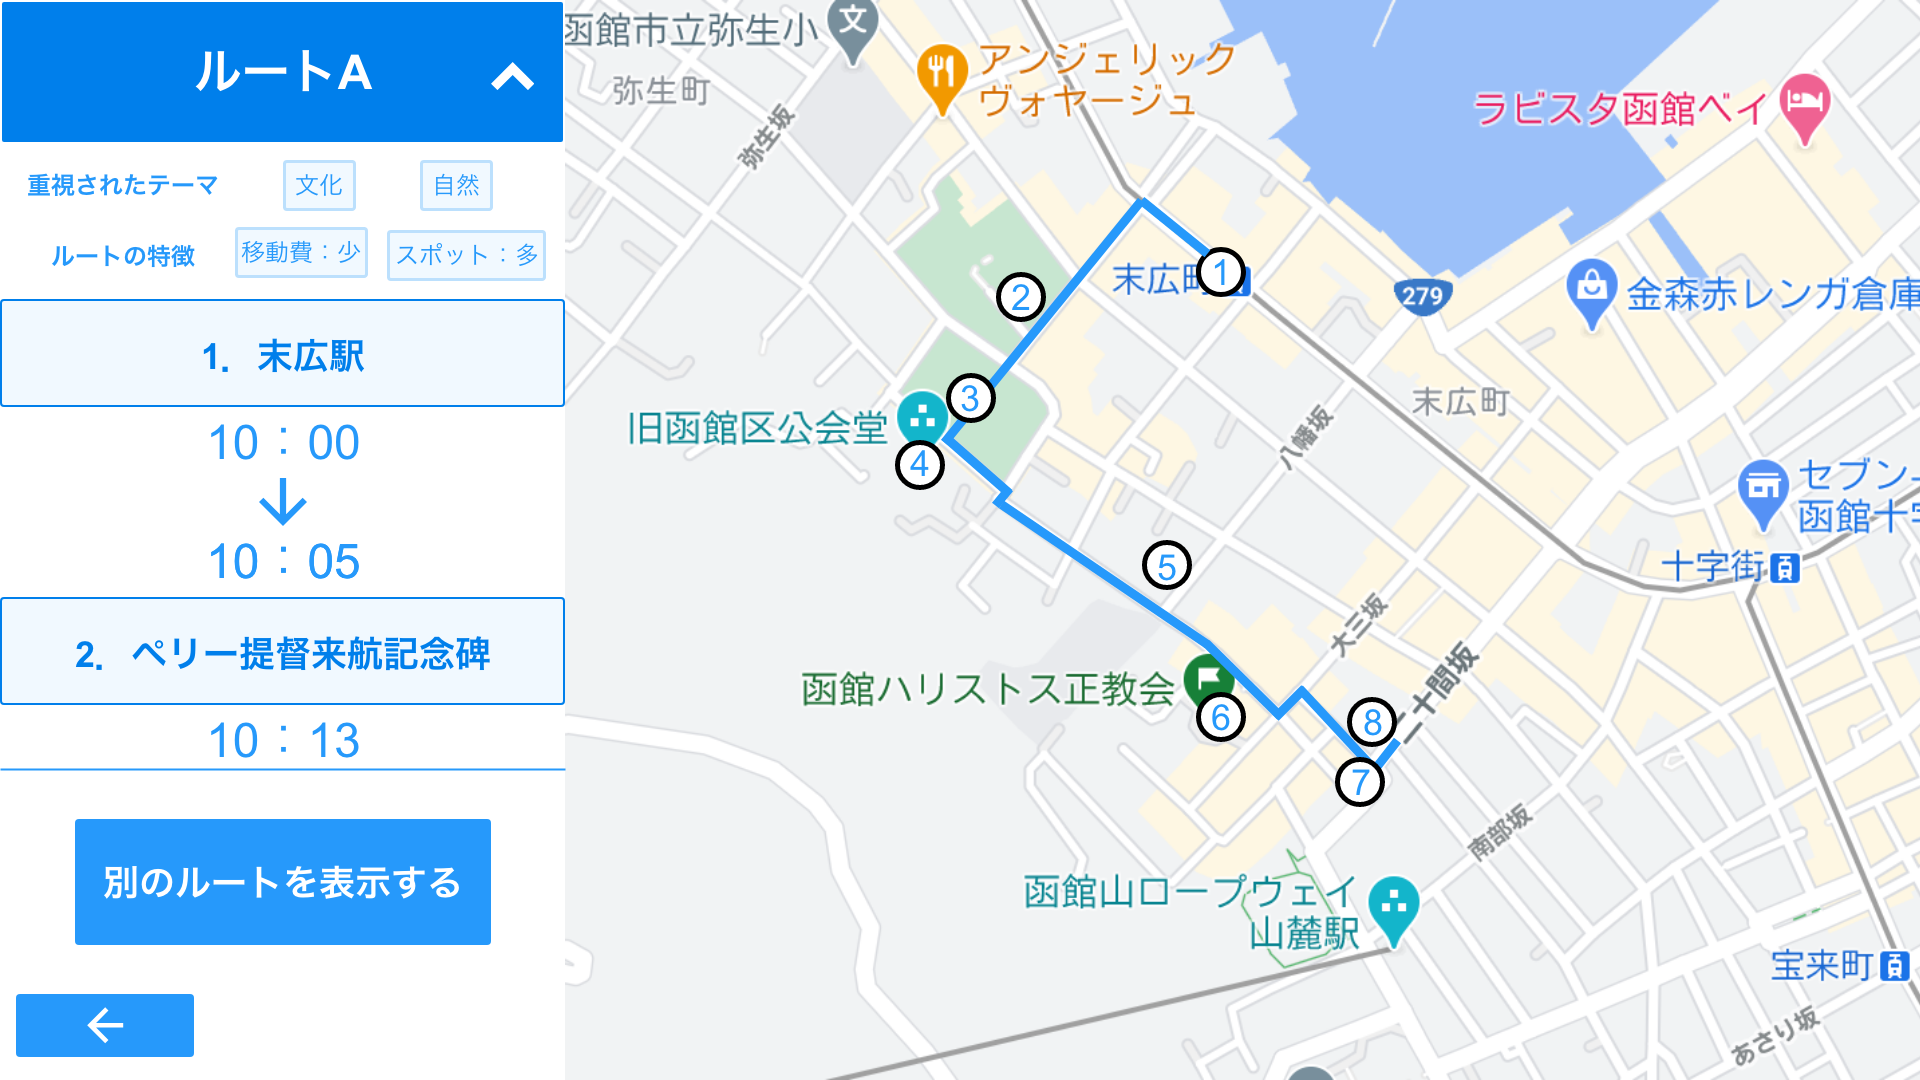
\includegraphics[width=8.5cm,bb=0 0 1980 1080]{sysimage1.png}
  \end{center}
  \caption{観光ルート表示画面} 
  \label{fig:観光ルート表示画面}
\end{figure}
\section{観光ルート自動生成アルゴリズム}\label{sec:観光ルート自動生成アルゴリズム}
本研究では,観光スポットと移動経路に対するユーザの嗜好を反映したルートの自動生成を行う.
そのために,Debらが提案した進化的遺伝的アルゴリズムであるNSGA-I\hspace{-.1em}I\hspace{-.1em}I\cite{NSGA3}とそれらの手法の解に対して任意の特徴を改善できる岸上らの研究\cite{岸上}を基にアルゴリズムを作成する.
NSGA-Ⅲは,遺伝的アルゴリズムを多目的最適化問題に適用できるように拡張したNSGA-I\hspace{-.1em}I\cite{NSGA2}に,reference pointの概念を加えたものである.
reference pointは解の検索方向を決める点である.
これを探索空間上に均一に配置することにより解の多様性を確保することができる.
また,任意の位置に配置することにより,特定の嗜好方向に特化した探索ができる.
以下に本研究におけるアルゴリズムの流れを記述する.
\subsection{初期個体の作成}\label{sec:初期解の作成}
% まず初めに,観光スポット全体からランダムに観光スポットを選択する.
% その際,ユーザの嗜好に合致している観光スポットが選ばれやすいようにする.
% 選択する観光スポット数は,観光に利用する時間に応じて一定の範囲からランダムに決定する.
% その後,選択した観光スポットを結ぶ最短経路をダイクストラ法を用いて求め,その経路を1つの初期個体とする.
% 一般に観光ルートを作成する場合,最短経路になるように作成することが多い.
% そのため,
まず初めに,観光スポット全体からランダムに観光スポットを選択し,それらを最短経路で結ぶ.
その際,ユーザの嗜好に合った観光スポットが選ばれやすいようにする.
また,初期個体を作成する段階で最短経路を求めることにより,初期個体が優秀になりやすくなる.
これらを初期個体数の数だけ行う.
\subsection{交叉}\label{sec:交叉}
次に,作成した個体を組み合わせて新たな個体を作成する.
個体同士の組み合わせには一点交叉を用いる.
交叉する親個体の選択は,様々な特徴を交叉するために,reference pointをランダムに選択し,それに対応する個体の中から選択する.
片方の親個体は,PBI距離がより大きな個体が選択されやすくする.
PBI距離とは,ある個体とそれに対応するreference line(原点とreference pointを結ぶ直線)までの最短距離を,原点からその交点までの距離から減算した値である.
もう一方の親個体は,PBI距離に加えて,先ほど選択した親個体と組み合わせる部分の距離も考慮する.
これにより,より優秀な解が生まれやすくなる.
\subsection{変異}\label{sec:変異}
次に,変異を行う初期個体をランダムに選択する.
変異の方法は平野らの研究\cite{平野}と同様に,増加変異と減少変異のどちらかをランダムに行う.
増加変異では,個体内の観光スポット間のいずれかの位置にランダムな観光スポットを追加する.
減少変異では,個体内の観光スポットのいずれかを削除する.
\subsection{淘汰}\label{sec:淘汰}
次に,初期個体と交配した個体,突然変異した個体からより優秀な個体を次世代に残す.
そのために,各reference pointに対応する個体から同数の個体が選択されるようにする.
その際,PBI距離が最も大きな個体から順に選択する.
これにより,多様性のある個体を次世代に残すことができる.
\subsection{ユーザによる解の評価}\label{sec:ユーザによる解の評価}
\ref{sec:交叉}節から\ref{sec:淘汰}節を規定の世代になるまで行う.
その後,reference pointからいくつかをランダムに選択し,それぞれに関連する個体の中で該当する最もPBI距離が大きい個体を表示する.
この際,ルートの改善が指示された場合,\cite{岸上}の原点を移動させる方法を用いて,一部の特徴を改善した解を生成するために,追加で\ref{sec:交叉}節から\ref{sec:淘汰}節を再度規定の世代になるまで行う.
その後,再度ユーザに選択された個体を表示する.
これをユーザが満足するまで行う.
% \ref{sec:観光ルート自動生成システム}節
% 本研究では,観光ルートを生成する際に観光スポットと移動経路に対するユーザの嗜好を反映したルートの自動生成を行う.
% そのために,Debらが提案した進化的遺伝的アルゴリズムであるNSGA-I\hspace{-.1em}I\hspace{-.1em}Iと,そこで用いられている reference line の概念を用いた岸上らの研究を参考にアルゴリズムを作成する.
% 以下にアルゴリズムの流れを記述する.

% \subsection{事前準備}\label{sec:事前準備}
% まず始めに,各観光スポット毎に「自然」や「文化」などのテーマにどの程度該当するかを決定する.
% また,ユーザにアンケートを実施し,観光スポットや移動経路に対する嗜好を推定する.
% その後,観光の開始・終了地点,開始・終了時間を設定してもらう.
		
% \subsection{初期解の作成}\label{sec:初期解の作成}
% 次に,1つの世代が有する解(観光ルート)の数Nを定義し,その数だけ観光ルートを作成する.
% 観光ルートを生成する手順は以下の通りである.
% \begin{enumerate}
%     \item 観光スポット全体からいくつかの観光スポットを選択する.
%     \item その際,選択する観光スポット数の範囲は開始・終了時間に合わせて相対的に変更する.
%     \item また,観光スポットはユーザの観光スポットに対する嗜好に合致するほど選択されやすくする.
%     \item 選択された観光スポットを最短距離で結ぶルートをダイクストラ法を用いて求め,それを1つの解とする.
% \end{enumerate}
% これらの手順を繰り返し行い,N個の解を生成する

% \subsection{交配}\label{sec:交配}
% まず,事前に定義した reference point と,ユーザのアンケート結果から定義した reference point に,2で作成した解を1つずつ関連づける.
% 関連づけは,解とその解との垂直距離が最も短い reference line (原点と reference point を結んだ直線)に対して行う.
% その後, reference line から1つをランダムに選択する.
% 選択された reference line に関連づけされた解が2つ以上ある場合,ランダムに2つを選択する.
% その後,選択した解のinvertedPBIを比較し,その値が大きい解を親Aとする.
% 解が1つである場合は,その解を親Aとする.
% 解が存在しなかった場合,全ての解の中から垂直距離が最も短い解を親Aとする.	
% ここで,親Aの観光スポット間をランダムに1つカットポイントとして設定する.
% その後同様に reference line をランダムに1つ選択し,関連づけされた解からランダムに2つを選択する.
% それら2つの解に対して親Aと同様にカットポイントを設定する.
% ランダムに選ばれた解のinvertedPBIと,親Aとそれぞれの解のカットポイントを結び付けた際の最短経路の距離の和を考慮し,どちらか一方の解を親Bとする.
% 親A,Bをカットポイントで結合し,新たな解を作成する.

% \subsection{突然変異}\label{sec:突然変異}
% まず,親の解からランダムに1つを選択する.
% 次に増加変異,もしくは減少変異のどちらかをランダムに選択する.
% 増加変異の場合,ランダムに観光スポット1つを選択し,それを観光スポット間のランダムな位置に追加する.
% 減少変異の場合,ランダムに観光スポットを1つ削除する.

% \subsection{生存競争}\label{sec:生存競争}
% 生存競争を行う前に,交配,突然変異で生成された解それぞれを reference line と関連づけする.
% その後, reference line をランダムに1つ選択する.
% その reference line に関連づけられている解の中からinvertedPBIが最も高い解を選択する.
% 選択した解を次の世代に引き継ぎ,選択された解の reference line との関連づけを削除する.
% 既に選択されたリファレンス以外から上記の手順を繰り返す.
% 全ての reference line が選択されたら,再度全ての reference line に対して,上記の手順を行う.
% 次世代の解の数がNに達した時点で終了する.

% \subsection{ユーザによる解の評価}\label{sec:ユーザによる解の評価}
% ここまでの\ref{sec:初期解の作成}節から\ref{sec:生存競争}節までを規定の世代に達するまで行う.
% その後,各 reference line からいくつかをランダムに選択し,それぞれに関連づけられている解の中からinvertedPBIが最も大きな解を選択する.
% 選択された解をユーザに表示し,下記のいずれかを行ってもらう.
% \begin{itemize}
%     \item 表示したコースに決定する
%     \item 他の解を表示する
%     \item 表示したコースの改善したい箇所を選択し,ルートの生成を追加で行う
%   \end{itemize}
% 「他の解を表示する」が選択された場合,まだ選ばれていない reference line から同様に解を選択し,ユーザに表示する.
% 「表示したコースの改善したい箇所を選択し,ルートの生成を追加で行う」が選択された場合,表示されているコースから好みのコースを選択する.
% その後,ルートの改善して欲しい箇所をチェックボックスを用いて選択する.
% 選択された改善箇所を基に原点を移動させ,再び\ref{sec:交配}節から規定の世代数に達するまで解の生成を繰り返す.

\section{アルゴリズムの評価}\label{sec:アルゴリズムの評価}
\ref{sec:観光ルート自動生成アルゴリズム}章のアルゴリズムを用いて,観光ルート推薦システムを構築し,有用性を検証するために評価実験を行う.
評価方法として,被験者を半数に分け,片方がWebサイトやSNSなどを用いて観光ルートを作成した後に,提案手法で観光ルートを作成する.
もう片方は逆の順番で観光ルートを作成する.
その後,被験者にどちらの観光ルートを利用したいかアンケートを実施する.
さらに,抽出した嗜好の中で,ユーザが重要視した評価項目に着目した定性的な比較評価も行う予定である.

\section{まとめ}\label{sec:まとめ}
本研究では,進化的遺伝的アルゴリズムであるNSGA-I\hspace{-.1em}I\hspace{-.1em}Iを用いて,観光スポットと移動経路に対するユーザの嗜好を反映したルートの自動生成とその評価を行う.
今後は\ref{sec:観光ルート自動生成アルゴリズム}章で述べたアルゴリズムを実装し,評価実験を行う.
その後,評価実験の結果を基にアルゴリズムの改善を行う.

% \section{はじめに}
% 情報処理学会北海道支部ではかねてより、情報処理北海道シンポジウムに
% 投稿される皆様の便宜をはかるために\LaTeX 用標準スタイルファイルを作成し、
% 皆様に配布することに致しました。

% この原稿は情報処理学会北海道支部から配布されるシンポジウム原稿作成
% 要領を\LaTeX によって作成したもので、シンポジウム用標準スタイルファ
% イルの使用例にもなっております。これを、よく御覧になったうえで、原稿を
% \underline{締切}までに作成されますようお願い致します。

% \section{どのようにして入手するか}
% スタイルファイルおよび申込書の\LaTeX ファイルは、情報処理学会北海道支部
% WWWホームページから入手できます。

% http://www.ipsj.or.jp/sibu/hokkaido/

% ブラウザから直接ダウンロードできるファイルは以下の4種類で、
% 漢字コード別に用意されています。
% \begin{enumerate}
% \item info.sty (原稿用スタイルファイル)
% \item sample.tex (この原稿の\LaTeX ファイル)
% \item form.tex (申込書の\LaTeX ファイル)
% \item form.sty (form.texのためのマクロ)
% \end{enumerate}

% \begin{figure}[h]
% \vspace{6.5cm}
% \caption{図は標準のパラメータより柔軟な配置ができるように設定してあります}
% \label{f1}
% \end{figure}

% \section{原稿の作成要領}

% \subsection{原稿の作成}
% 原稿の例はsample.tex(このファイル)に入っています。これを\LaTeX にかけることで
% 見本原稿が出来上がります。\LaTeX 以外で原稿を作成する場合は、この見本の寸法を
% 参考にして上下左右のマージンをとって下さい。

% \LaTeX で原稿を作成する場合は、sample.texを編集して原稿を作成して下さい。
% このスタイルファイルでは、Emailコマンドを指定することで著者のメールアドレスが、また、
% contacttoコマンドを指定することで連絡先の住所が、自動的に第1頁のフットノートとして記
% 入されます。

% もし、プリンタでの印刷位置が左右のどちらかにずれてしまう場合には、info.styファ
% イルの先頭にある水平オフセットの量を調整してみて下さい。

% \subsection{申込書の作成}
% 申込書はform.texというファイルと、form.styというマクロから作られます。
% このファイルをそのまま\LaTeX にかけますと、見本の申込書と同時に
% 申込要領が作成されます。

% つぎに、form.texのコメント文字列(\%\%$\ldots$\%\%)ではさまれた部分に見本として記
% 入された著者名や論文題名などのデータを、各自の原稿に合うように編集して下さい。これを
% \LaTeX にかけると提出用の申込書の出来上がりです。

% もし、手書き用の申し込み用紙を作成したい場合は、これらの著者名や論文題名などの
% データを定義するコマンドの行頭にコメントマーク(\% )を入れて\LaTeX にかけてください。

% \section{まとめ}
% 以上、情報処理学会北海道支部で作成したスタイルファイルと申込書の使い方を説明し
% てきました。このファイルを皆様の研究に役立てていただけますなら、作成者冥利に
% 尽きるというものです。

\begin{thebibliography}{99}
\bibitem{倉田} 倉田陽平:CT-Planer 3:Web上での対話的な旅行プラン作成支援,観光科学研究,5,pp.159-165(2012)
\bibitem{平野} 平野陽大,諏訪博彦,安本慶一:ユーザのリソース消費を考慮した意思決定支援のための複数観光経路提示手法,情報処理学会,マルチメディア,分散協調とモバイルシンポジウム2019論文集,pp.830-839(2019)
\bibitem{NSGA2} K. Deb,A. Pratap,S.Agarwal,T.Meyarivan.:A fast and elitist multiobjective genetic algorithm: NSGA-I\hspace{-.1em}I,IEEE Transactions on Evolutionary Computation,Vol.6,pp.182-197(2002)
\bibitem{NSGA3} K. Deb,H. Jain:An evolutionary many-objective optimization algorithm using reference-point-based nondominated sorting approach, part I: Solving problems with box constraints,IEEE Transactions on Evolutionary Computation,Vol.18,pp.577-601(2014)
\bibitem{岸上} 岸上利裕,吉川大弘:reference lineに基づくユーザの嗜好方向探索手法の提案,進化計算学会論文誌,Vol.6,pp.31-41(2015)
\end{thebibliography}
\end{document}
%
%
% End of file: sample.tex
